\subsection{System Equations}


The equation for a ball on a beam was taken from the material from the first lab in the course, and can be written as

\begin{equation}
m(\ddot{x}-x\dot{\phi}^{2})=-mg\sin(\phi)-\frac{2}{5}m\ddot{x},
\end{equation}
where $x$ is the distance of the ball along the beam, $m$ is the mass of the ball and $\phi$ is the angle of the beam.

We chose a simple model for the beam, letting the control signal be proportional to the torque on the beam.
To account for the displacement of the beam around the rotational center, we modeled a force proportional to the angle of the beam.
This approximation turned out to be quite good, especially for small angles.
The last part of this model is the force applied to the beam by the ball.
The differential equation is given as
\begin{equation}
J_{B}\ddot{\phi}=k_{u}u+mgx\cos(\phi)+k_B\phi,
\end{equation}
where $J_{B}$ is the moment of inertia of the beam, $k_u$ is the torque to control signal ratio and $k_B$ the estimated torque per radian from the displacement of the beam.\\
\\
Letting $x_{1}=x,\, x_{2}=\dot{x},\, x_{3}=\phi,\, x_{4}=\dot{\phi}$,
we can then write the system as a set of first order nonlinear differential equations

%\begin{eqnarray*}
%m(\dot x_{2}-x_{1}x_{4}^{2}) & = & -mg\sin(x_{3})-\frac{2}{5}m\dot{x}_{2}\\
% & \Leftrightarrow\\
%\dot{x}_{2} & = & \frac{5}{7}\left(-g\sin(x_{3})+x_{1}x_{4}^{2}\right)
%\end{eqnarray*}
%
%
%and beam equation as
%\[
%\dot{x}_{4}=\frac{1}{J_B}\left(k_{u}u+mgx_{1}\cos(x_3)+k_Bx_3\right).
%\]
%
%
%We thus have then nonlinear first order system equations

\[
\begin{pmatrix}\dot{x}_{1}\\
\dot{x}_{2}\\
\dot{x}_{3}\\
\dot{x}_{4}
\end{pmatrix}=\begin{pmatrix}x_{2}\\
\frac{5}{7}\left(-g\sin(x_{3})+x_{1}x_{4}^{2}\right)\\
x_{4}\\
\frac{1}{J_B}mgx_{1}\cos(x_3)+\frac{k_B}{J_B}x_3
\end{pmatrix}+\begin{pmatrix}0\\
0\\
0\\
\frac{k_{u}}{J_B}
\end{pmatrix}u.
\]

\subsection{Linearization}

We introduced the mass of the ball as a state $x_{5}=m$ in the system. The advantage of this is that it would then be possible to start estimating the weight of the ball earlier in the sequence.
It would also allow feed forward to the control signal based on the mass and position of the ball, this could have greatly reduced the oscillations of the beam control since we would not require integral action to account for this entire force.
We lastly introduced the integral of the deviation of the position of the
ball $(\tilde{x}_{6}=\int_{0}^{t}\tilde{x}_{1}dt)$ as a state and linearized the system around the steady state $\bar{x}=(\bar{x}_{1},0,0,0,\bar{m},\bar{u})$.
This results in the linear perturbation equations
%\begin{eqnarray*}
%\dot{\tilde{x}} & = & \begin{pmatrix}0 & 1 & 0 & 0 & 0\\
%\frac{5}{7}\bar{x}_{4}^{2} & 0 & -\frac{5g}{7}\cos(\bar{x}_{3}) & 2\bar{x}_{1}\bar{x}_{4} & 0\\
%0 & 0 & 0 & 1 & 0\\
%\bar{m}\frac{g}{J_B}\cos(\bar{x}_{3}) & 0 & -\bar{m}\frac{g}{J_B}\bar{x}_{1}\sin(\bar{x}_{3})+\frac{k_B}{J_B} & 0 & \frac{g}{J_B}\bar{x}_{1}\cos(\bar{x}_{3})\\
%0 & 0 & 0 & 0 & 0
%\end{pmatrix}\tilde{x}+\begin{pmatrix}0\\
%0\\
%0\\
%\frac{k_{u}}{J_B}\\
%0
%\end{pmatrix}\tilde{u}\\
% & = & \begin{pmatrix}0 & 1 & 0 & 0 & 0\\
%0 & 0 & -\frac{5g}{7} & 0 & 0\\
%0 & 0 & 0 & 1 & 0\\
%\bar{m}\frac{g}{J_B} & 0 & \frac{k_B}{J_B} & 0 & \frac{g}{J}\bar{x}_{1}\\
%0 & 0 & 0 & 0 & 0
%\end{pmatrix}\tilde{x}+\begin{pmatrix}0\\
%0\\
%0\\
%\frac{k_{u}}{J_B}\\
%0
%\end{pmatrix}\tilde{u}.
%\end{eqnarray*}

\begin{eqnarray*}
\dot{\tilde{x}} & = & \begin{pmatrix}0 & 1 & 0 & 0 & 0 & 0\\
0 & 0 & -\frac{5g}{7} & 0 & 0 & 0\\
0 & 0 & 0 & 1 & 0 & 0\\
\bar{m}\frac{g}{J_B} & 0 & \frac{k_B}{J_B} & 0 & \frac{g}{J_B}\bar{x}_{1} & 0\\
0 & 0 & 0 & 0 & 0 & 0\\
1 & 0 & 0 & 0 & 0 & 0
\end{pmatrix}\tilde{x}+\begin{pmatrix}0\\
0\\
0\\
\frac{k_{u}}{J_B}\\
0\\
0
\end{pmatrix}\tilde{u}\\
 & = & A\tilde{x}+B\tilde{u}\\
\tilde{y} & = & \begin{pmatrix}1 & 0 & 0 & 0 & 0 & 0\\
0 & 0 & 1 & 0 & 0 & 0
\end{pmatrix}\tilde{x}+w=C\tilde{x}
\end{eqnarray*}
where $\tilde{x}=x-\bar{x}$, $\tilde{u}=u-\bar{u}$.
\\
The system is now in a form that works with the LQG framework.

%where $v$ and $w$ has intensity matrices $V$ and $W$. We now define
%the cost function $J=E\left[\int_{0}^{\infty}\tilde{x}^{T}Q\tilde{x}^{T}+u^{T}\frac{1}{r^{2}}u\, dt\right]$,
%with $Q=\text{diag}\left(\frac{1}{q_{1}^{2}},\frac{1}{q_{2}^{2}},\frac{1}{q_{3}^{2}},\frac{1}{q_{4}^{2}},\frac{1}{q_{5}^{2}}\right)$
%and let the controller be

%\begin{eqnarray*}
%\dot{\hat{x}} & = & A\hat{x}+B\tilde{u}+K(y-C\hat{x})\\
%\tilde{u} & = & -L\hat{x}.
%\end{eqnarray*}


%The optimal $K$ and $L$ is then given by the symmetric positive
%definite solutions $P$ and $S$ to 
%\begin{eqnarray*}
%0 & = & AP+PA^{T}-PC^TW^{-1}CP+V\\
%0 & = & A^{T}S+SA-SBR^{-1}B^{T}S+Q
%\end{eqnarray*}


%as $K=PC^{T}W^{-1}$ and $L=R^{-1}B^{T}S$.

%An initial guess for the matrices $Q$ and $R$ could be given by
%giving similar penalty for deviations $(3cm,1cm/s,2^{\circ},0.5^{\circ}/s,-,20cm\cdot s)$
%and $(1V)??$. Thus

%$Q=\text{diag}(1111,10000,816,13131,0,25)$, $R=1.$


\subsection{Throw Equations}

To be able to throw the ball to a desired location we needed to know how the relation between the terminal state of the ball on the beam and the distance traveled in the air.
We derived this relation using the nonlinear system equations above and the equations for a free falling body.
The resulting equations are

%\begin{eqnarray*}
%h & = & h_{0}+v_{y_{0}}t-\frac{gt^{2}}{2}\\
%d & = & d_{0}+v_{x_{0}}t,
%\end{eqnarray*}


%which results in the terminal time $t_{T}=(d_{T}-d_{0})/v_{x_{0}}$.

%We desire 
%\begin{eqnarray*}
%h_{T} & = & -d_{y}\\
%d_{T} & = & d_{x},
%\end{eqnarray*}


%and know
%\begin{eqnarray*}
%h_{0} & = & l\sin(\phi)\\
%d_{0} & = & l\cos(\phi),
%\end{eqnarray*}


%which gives
%\begin{eqnarray*}
%-d_{y} & = & l\sin(\phi)+v_{y_{0}}t-\frac{gt^{2}}{2}\\
%d_{x} & = & l\cos(\phi)+v_{x_{0}}t.
%\end{eqnarray*}


%The velocity of the ball in the horizontal and vertical directions
%are
%\begin{eqnarray*}
%v_{x} & = & \dot{x}\cos(\phi)-x\dot{\phi}\sin(\phi)\\
%v_{y} & = & \dot{x}\sin(\phi)-x\dot{\phi}\cos(\phi),
%\end{eqnarray*}


%and at the release-time, we have $x=l$. These equations gives
\begin{eqnarray*}
-d_{y}(t) & = & l\sin(\phi)+\left(\dot{x}\sin(\phi)-l\dot{\phi}\cos(\phi)\right)t-\frac{gt^{2}}{2}\\
d_{x}(t) & = & l\cos(\phi)+\left(\dot{x}\cos(\phi)-l\dot{\phi}\sin(\phi)\right)t,
\end{eqnarray*}
where $d_{y}(t), d_{x}(t)$ are the distances traveled after time $t$ as given in Figure \ref{fig:throw} and $(x=l,\dot x,\phi, \dot{\phi})$ is the state when the ball is leaving the beam.

\begin{figure}[\textwidth]
\centering
\begin{tikzpicture}[scale=1.5]
\usetikzlibrary{patterns,snakes}
\definecolor{Darkgreen}{rgb}{0,0.4,0}
\tikzstyle{brace} = [decorate, decoration={brace, amplitude=5pt}]

\node[inner sep=0] (v0) at (0,0) {};
\node[inner sep=0] (v2) at (2,0.5) {};
\node[inner sep=0] (v1) at (-1,-0.25) {};

\draw[color=red]  (v1) edge (v2);

\node (v3) at (8,-2) {};
\node (v4) at (0,-2) {};
\node (v5) at (8,0) {};

\draw[ball color=blue] (2,0.6) circle (.1);

\draw[dashed,->] (v2) -- (4,1) node[pos=1,above] {$\dot{x}$};
\draw[dashed] (v0) -- (v5) {};
\draw[dashed] (v0) -- (v4) {};
\draw[brace] (v0) -- (v2) node[pos=0.5,above,yshift=6] {$l=x$};
\draw[brace] (v3) -- (v4) node[pos=0.5,below,yshift=-6] {$d_x$};
\draw[brace] (v5) -- (v3)  node[pos=0.5,right,xshift=5] {$d_y$};

 \draw[color=green] plot[smooth] coordinates {(v2) (4,0.6) (6,0) (8,-2)};
 
 
\node at (1.3,0.17) {$\phi$};

\path[clip] (2,0.5) -- (0,0) -- (2,0);
\node[circle,draw=Darkgreen, minimum size=90pt] at (0,0) (circ) {};

\end{tikzpicture}
\caption{Illustration of the ball and its calculated trajectory as it is leaving the beam.}
\label{fig:throw}
\end{figure}
%
%and from the second equation we arrive at 
%\[
%t=\frac{\left(d_{x}-l\cos(\phi)\right)}{\dot{x}\cos(\phi)-l\dot{\phi}\sin(\phi)},
%\]
%

%and can thus insert that into the first equation:
%\begin{gather*}
%-d_{y}=l\sin(\phi)+\frac{\left(\dot{x}\sin(\phi)-l\dot{\phi}\cos(\phi)\right)\left(d_{x}-l\cos(\phi)\right)}{\dot{x}\cos(\phi)-l\dot{\phi}\sin(\phi)}-\frac{g}{2}\left(\frac{\left(d_{x}-l\cos(\phi)\right)}{\dot{x}\cos(\phi)-l\dot{\phi}\sin(\phi)}\right)^{2}.
%\end{gather*}

To be able to find a satisfactory terminal state we made the assumption of zero terminal angular velocity of the beam ($\dot{\phi}=0$). This allows us to explicitly solve for the relation between terminal ball velocity and angle of the beam as

%\subsection{Assuming $\dot{\phi}=0$}
%
%We can simplify the equation if we assume stationary beam at realease
%($\dot{\phi}=0$) 
%\begin{eqnarray*}
%-d_{y}\dot{x}^{2}\cos^{2}(\phi) & = & \dot{x}^{2}\cos^{2}(\phi)l\sin(\phi)+\dot{x}^{2}\cos(\phi)\sin(\phi)\left(d_{x}-l\cos(\phi)\right)-\frac{g}{2}\left(d_{x}-l\cos(\phi)\right)^{2}
%\end{eqnarray*}
%simplify:
%
%\[
%-d_{y}\dot{x}^{2}\cos^{2}(\phi)=\dot{x}^{2}\cos(\phi)\sin(\phi)d_{x}-\frac{g}{2}\left(d_{x}-l\cos(\phi)\right)^{2}
%\]
%
%
%and we can then finally solve for $\dot{x}$:
%
\[
\dot{x}=\left(d_{x}-l\cos(\phi)\right)\frac{\sqrt{g}}{\sqrt{2\cos(\phi)\left(d_{y}\cos(\phi)+d_{x}\sin(\phi)\right)}}.
\]

Given a fix $d_x,d_y$ it is now possible to find a pair of $\dot x,\phi$ to which we could generate a trajectory using the iterative gradient based method described in \cite{NR}, chapter 21.1.1.

One example of a generated trajectory for the process using this framework can be seen in Figure \ref{fig:matlabtrajectory}.

\begin{figure}[\textwidth]
\centering
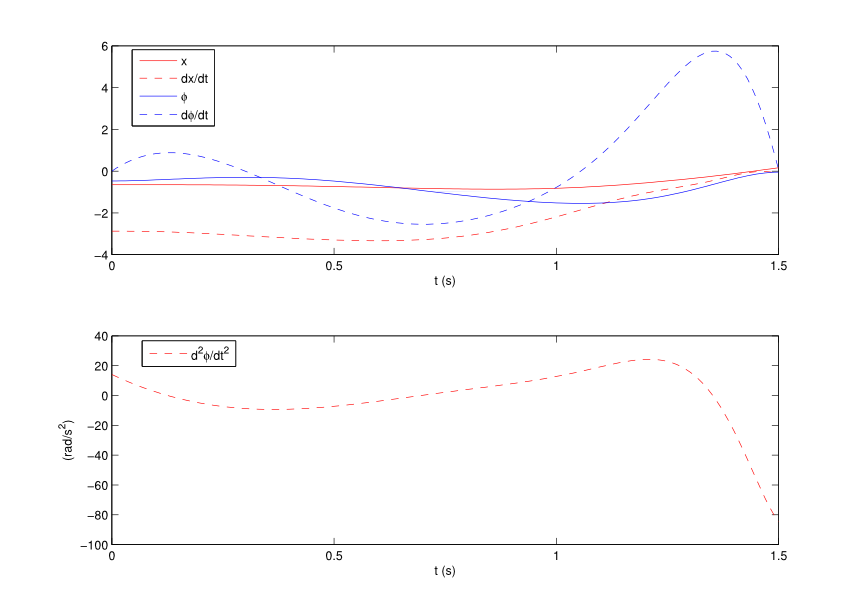
\includegraphics[width=\textwidth]{ballbeammatlab}
\caption{Example of trajectory generated using the gradient based iterative optimization. The states are plotted as deviations from the desired terminal condition. The second derivative of the angular velocity of the beam is used as control signal in this example, that that could easily be recalculated to the force required by the controller using the model.}
\label{fig:matlabtrajectory}
\end{figure}